\documentclass[class=scrreprt]{standalone}

\usepackage{amssymb}
\usepackage{bm}
\usepackage{pgfplots}
\pgfplotsset{compat=newest}
\usepgfplotslibrary{groupplots}

\KOMAoptions{fontsize=9pt}


  \begin{document}
  \begin{tikzpicture}
\draw[white](0,0) rectangle (12,6.5);
	\begin{axis}[at={(1cm,0.5cm)},
	width=6cm,
	height=5.25cm,
	view={105}{15},
	    scale only axis=true,
            enlargelimits=false,
	    axis lines=center,
            xmin=0,
            xmax=1.01,
            xtick={0,0.25,0.5,0.75,1},
            xticklabels={\empty},
            ymin=0,
            ymax=1.01,
            ytick={0,0.25,0.5,0.75,1},
            yticklabels={\empty},
	 zmin = 0,
	 zmax = 325,
            ztick={0,100,200,300},
            zticklabels={\empty},	
            xmajorgrids=true,
            ymajorgrids=true,
            grid,]


	\addplot3[color=black!50!white,very thin] coordinates {(0.25,0,0) (0.25,1,0)};
	\addplot3[color=black!50!white,very thin] coordinates {(0.5,0,0) (0.5,1,0)};
	\addplot3[color=black!50!white,very thin] coordinates {(0.75,0,0) (0.75,1,0)};
	\addplot3[color=black!50!white,very thin] coordinates {(1,0,0) (1,1,0)};
	\addplot3[color=black!50!white,very thin] coordinates {(0,0.25,0) (1,0.25,0)};
	\addplot3[color=black!50!white,very thin] coordinates {(0,0.5,0) (1,0.5,0)};
	\addplot3[color=black!50!white,very thin] coordinates {(0,0.75,0) (1,0.75,0)};
	\addplot3[color=black!50!white,very thin] coordinates {(0,1,0) (1,1,0)};
	
	\addplot3[color=black!50!white,very thin] coordinates {(0,0,100) (0,1,100)};
	\addplot3[color=black!50!white,very thin] coordinates {(0,0,200) (0,1,200)};
	\addplot3[color=black!50!white,very thin] coordinates {(0,0,300) (0,1,300)};
	
	\addplot3[color=black!50!white,very thin] coordinates {(0,0.25,0) (0,0.25,325)};
	\addplot3[color=black!50!white,very thin] coordinates {(0,0.5,0) (0,0.5,325)};
	\addplot3[color=black!50!white,very thin] coordinates {(0,0.75,0) (0,0.75,325)};
	\addplot3[color=black!50!white,very thin] coordinates {(0,1,0) (0,1,325)};
	
	
	\addplot3[color=black!50!white,very thin] coordinates {(0.25,0,0) (0.25,0,325)};
	\addplot3[color=black!50!white,very thin] coordinates {(0.5,0,0) (0.5,0,325)};
	\addplot3[color=black!50!white,very thin] coordinates {(0.75,0,0) (0.75,0,325)};
	\addplot3[color=black!50!white,very thin] coordinates {(1,0,0) (1,0,325)};
	
	\addplot3[color=black!50!white,very thin] coordinates {(0,0,100) (1,0,100)};
	\addplot3[color=black!50!white,very thin] coordinates {(0,0,200) (1,0,200)};
	\addplot3[color=black!50!white,very thin] coordinates {(0,0,300) (1,0,300)};
        	
	\addplot3[
            mesh/rows=101,
            mesh/cols=101,
            surf,  
	 shader= interp,
            colormap/viridis,  
            point meta min= 0,   
            point meta max=  315,
            ] table[x=a, y=b, z=c] from {Compliance_minimization/Figure_3/2d_projection.txt};
	\addplot3 [very thin, black, opacity=0.5,
            ] table[x=a, y=b, z=c] from {Compliance_minimization/Figure_3/2d_mesh.txt};
	\addplot3 [thin, black,
            ] table[x=a, y=b, z=c] from {Compliance_minimization/Figure_3/2d_mesh_2.txt};
              
	\end{axis}
	\node at (1.15,0.65) {$a$};
	\node at (7.15,1.45) {$b$};
	\node at (2.5,5.75) {$C$};
	\node at (6.8,1.67) {$1$};
	\node at (0.9,0.95) {$1$};
	\node[right] at (2.2,1.95) {$0$};
	\node[right] at (2.2,5.25) {$300$};
	
	\node[black,thin,left] at (1,5.7) {\textbf{A}};
             \begin{scope}[scale=0.6,xshift=13.33cm, yshift=7.5cm]
                 \node[] at (2.5,1.25)
                     {
\includegraphics[width=3cm]{Compliance_minimization/Figure_3/vis_1_X1.png}};
	\draw[step=0.0555555cm,black!50!white, very thin,shift={(0,0)}] (0,0)  grid(5,2.5);
                 \draw[black,thin] (0,0) rectangle(5,2.5);% Bearings
                 \draw[black,thin] (4.75,-0.25) -- (5,0) -- (5.25,-0.25)--  cycle;
                 \draw[black,thin] (4.75,-0.5) -- (5.25,-0.5);
                 \draw[black,thin] (4.75,-0.6)--(4.85,-0.5);
                 \draw[black,thin] (4.85,-0.6)--(4.95,-0.5);
                 \draw[black,thin] (4.95,-0.6)--(5.05,-0.5);
                 \draw[black,thin] (5.05,-0.6)--(5.15,-0.5);
                 \draw[black,thin] (5.15,-0.6)--(5.25,-0.5);
                 \draw[black,thin] (5.125,-0.375) circle(0.125);
                 \draw[black,thin] (4.875,-0.375) circle(0.125);

                 \draw[black,thin] (-0.25,0)--(-0.25,2.5);
                 \draw[black,thin] (-0.35,0)--(-0.25,0.1);
                 \draw[black,thin] (-0.35,0.1)--(-0.25,0.2);
                 \draw[black,thin] (-0.35,0.2)--(-0.25,0.3);
                 \draw[black,thin] (-0.35,0.3)--(-0.25,0.4);
                 \draw[black,thin] (-0.35,0.4)--(-0.25,0.5);
                 \draw[black,thin] (-0.35,0.5)--(-0.25,0.6);
                 \draw[black,thin] (-0.35,0.6)--(-0.25,0.7);
                 \draw[black,thin] (-0.35,0.7)--(-0.25,0.8);
                 \draw[black,thin] (-0.35,0.8)--(-0.25,0.9);
                 \draw[black,thin] (-0.35,0.9)--(-0.25,1.0);
                 \draw[black,thin] (-0.35,1.0)--(-0.25,1.1);
                 \draw[black,thin] (-0.35,1.1)--(-0.25,1.2);
                 \draw[black,thin] (-0.35,1.2)--(-0.25,1.3);
                 \draw[black,thin] (-0.35,1.3)--(-0.25,1.4);
                 \draw[black,thin] (-0.35,1.4)--(-0.25,1.5);
                 \draw[black,thin] (-0.35,1.5)--(-0.25,1.6);
                 \draw[black,thin] (-0.35,1.6)--(-0.25,1.7);
                 \draw[black,thin] (-0.35,1.7)--(-0.25,1.8);
                 \draw[black,thin] (-0.35,1.8)--(-0.25,1.9);
                 \draw[black,thin] (-0.35,1.9)--(-0.25,2.0);
                 \draw[black,thin] (-0.35,2.0)--(-0.25,2.1);
                 \draw[black,thin] (-0.35,2.1)--(-0.25,2.2);
                 \draw[black,thin] (-0.35,2.2)--(-0.25,2.3);
                 \draw[black,thin] (-0.35,2.3)--(-0.25,2.4);
                 \draw[black,thin] (-0.35,2.4)--(-0.25,2.5);
                
                 \draw[black,thin] (-0.125,0.125) circle(0.125);
                 \draw[black,thin] (-0.125,0.375) circle(0.125);
                 \draw[black,thin] (-0.125,0.625) circle(0.125);
                 \draw[black,thin] (-0.125,0.875) circle(0.125);
                 \draw[black,thin] (-0.125,1.125) circle(0.125);
                 \draw[black,thin] (-0.125,1.375) circle(0.125);
                 \draw[black,thin] (-0.125,1.625) circle(0.125);
                 \draw[black,thin] (-0.125,1.875) circle(0.125);
                 \draw[black,thin] (-0.125,2.125) circle(0.125);
                 \draw[black,thin] (-0.125,2.375) circle(0.125);
                 \node[black,thin,right] at (5,2) {\textbf{B}};
             \end{scope} 
             \begin{scope}[scale=0.6,xshift=13.33cm, yshift=4.16666cm]
                 \node[] at (2.5,1.25)
                     {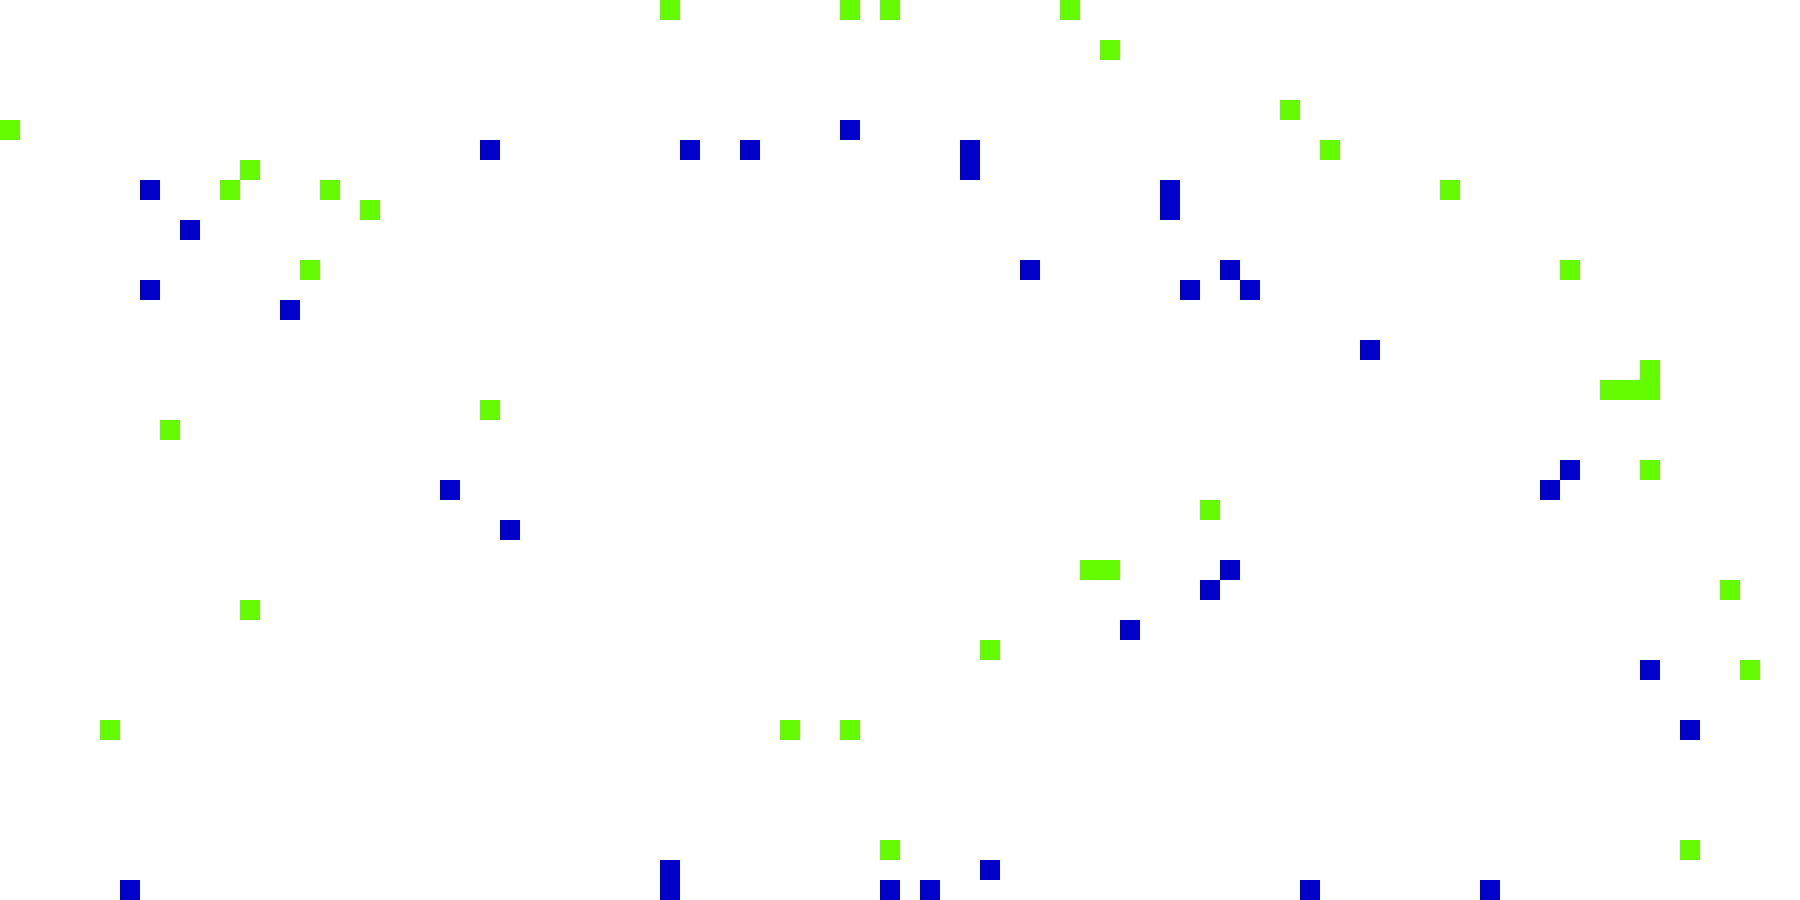
\includegraphics[width=3cm]{Compliance_minimization/Figure_3/vis_1_dX1.png}};
	\draw[step=0.0555555cm,black!50!white, very thin,shift={(0,0)}] (0,0)  grid(5,2.5);
                 \draw[black,thin] (0,0) rectangle(5,2.5);% Bearings
                 \node[black,thin,right] at (5,2) {\textbf{C}};
             \end{scope}
             \begin{scope}[scale=0.6,xshift=13.33cm, yshift=0.83333cm]
                 \node[] at (2.5,1.25)
                     {
\includegraphics[width=3cm]{Compliance_minimization/Figure_3/vis_1_dX2.png}};
	\draw[step=0.0555555cm,black!50!white, very thin,shift={(0,0)}] (0,0)  grid(5,2.5);
                 \draw[black,thin] (0,0) rectangle(5,2.5);% Bearings
                 \node[black,thin,right] at (5,2) {\textbf{D}};
             \end{scope}
 \end{tikzpicture}
 \end{document}